\begin{figure}[H]
\centering
\tikzset{arrow/.style={-stealth, thick, draw=gray!80!black}}

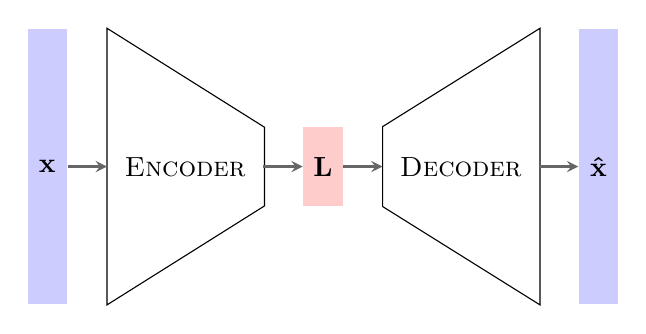
\begin{tikzpicture}
%     \draw[help lines](0,-5) grid (10,5);  
     
	\node[fill=blue!20, minimum width=0.5cm, minimum height=3.5cm] (X) at (0,0) {$\mathbf x$};
	
	\draw[fill=white!20] ([xshift=0.5cm]X.north east) -- ([xshift=2.5cm,yshift=0.5cm]X.east) -- ([xshift=2.5cm,yshift=-0.5cm]X.east) -- ([xshift=0.5cm]X.south east) -- cycle; 
	\node at (1.75,0) {\textsc{Encoder}};
	
	\node[fill=red!20, minimum width=0.5cm, minimum height=1.0cm] (Z) at (3.5cm,0) {$\mathbf L$};
	
	\draw[fill=white!20] ([xshift=0.5cm]Z.north east) -- ([xshift=2.5cm,yshift=1.25cm]Z.north east) -- ([xshift=2.5cm,yshift=-1.25cm]Z.south east) -- ([xshift=0.5cm]Z.south east) -- cycle;
	\node at (5.25,0) {\textsc{Decoder}};
	
	\node[fill=blue!20, minimum width=0.5cm, minimum height=3.5cm] (Xp) at (7,0) {$\mathbf{\hat{x}}$};
	
	\draw[arrow] (X.east) -- ([xshift=0.5cm]X.east);
	\draw[arrow] ([xshift=-0.5cm]Z.west) -- (Z.west);
	\draw[arrow] (Z.east) -- ([xshift=0.5cm]Z.east);
	\draw[arrow] ([xshift=-0.5cm]Xp.west) -- (Xp.west);
     
\end{tikzpicture}
\caption{Autoencoder, \cite{Autoencoder-tikz}} \label{fig:autoencoder}
\end{figure}
